% Author: CSC Officers
\documentclass[11pt]{article}
\usepackage{fullpage}
\usepackage{listings}
\usepackage{needspace}
\usepackage{color}
\usepackage{ifthen}
\usepackage{pgf}
\usepackage{tikz}
\usetikzlibrary{arrows,automata,shapes}
\usepackage{amsmath}
\usepackage{url}
\usepackage{framed}
\usepackage{csc}
\usepackage{textcomp}
\usepackage{multicol}

\lstset{ %
basicstyle=\footnotesize,       % the size of the fonts that are used for the code
numbers=left,                   % where to put the line-numbers
stepnumber=1,                   % the step between two line-numbers. If it's 1 each line will be numbered
numbersep=5pt,                  % how far the line-numbers are from the code
showspaces=false,               % show spaces adding particular underscores
showstringspaces=false,         % underline spaces within strings
tabsize=4,		                % sets default tabsize to 4 spaces
language=Python
}

\ifthenelse{\isundefined{\isAnswerKey}}
{
    \newenvironment{answer}{\large\lstset{basicstyle=\tiny}\color{white}}{}
}
{
    \newenvironment{answer}{\large\lstset{basicstyle=\large}\color{red}}{}
}

\title{CS-141 Exam 2 Review}
\author{Computer Science Community}
\date{\today}

\makeatletter
\let\thetitle\@title
\let\theauthor\@author
\let\thedate\@date
\makeatother

\begin{document}
\header

\begin{enumerate}

\section*{Linked Lists}
    \item You are given the linked list: $1 \rightarrow 2 \rightarrow 3$.  You may assume that each node has one field called \texttt{value} and one called \texttt{next}.
        \begin{enumerate}
            \item 1 points to 2 and 2 points to 3. What does 3 point to? \\
                \begin{answer}
				The implementer may cause the 3 node to point to either \texttt{None} or a sentinel node.
				\end{answer}
            \item Draw out the linked list structure and add a 5 to the end.
				\begin{answer}
				\leftmargin=0em
				\itemindent=0em
				{ \small
				\begin{verbatim}
+----------+    +----------+    +----------+    +------------+
| value: 1 |    | value: 2 |    | value: 3 |    | value: 5   |
| next: ------->| next: ------->| next: ------->| next: None |
+----------+    +----------+    +----------+    +------------+
				\end{verbatim}
				\textit{OR}
				\begin{verbatim}
+----------+    +----------+    +----------+    +----------+    +-----------------+
| value: 1 |    | value: 2 |    | value: 3 |    | value: 5 |    | value: SENTINEL |
| next: ------->| next: ------->| next: ------->| next: ------->|                 |
+----------+    +----------+    +----------+    +----------+    +-----------------+
				\end{verbatim} }
				\end{answer}
            \item Write pseudocode to add an element onto the end of a linked list.
				\begin{answer}
				\begin{lstlisting}
def append(value, linked_list):
	newend = new node
	newend.value = value
	newend.next = None # (or SENTINEL)
	curend = end node of linked_list
	curend.next = newend
				\end{lstlisting}
				\end{answer}
				\vspace{1in}
            \item Looking at the list from (b), you notice that we forgot to
                  add in a 4. What is a procedure for doing this? (There are
                  many possibilities.) \\
                \begin{answer}
				Use some variation of this strategy: Find the preceding element's node (in this case, 3), link its next node to the new node containing 4, then link that new node to what was the following node.
				\end{answer}
				\vspace{1in}
        \end{enumerate}

\pagebreak
\section*{Stacks and Queues}
	\item If we wanted to implement a stack as a linked list, what linked-list
	operations would correspond to \texttt{push()} and \texttt{pop()}?

	\begin{answer}
	\texttt{push( stack, element )} $\rightarrow$ \texttt{insertFront( linked-list, element )} \\
	\texttt{pop( stack )} $\rightarrow$ \texttt{removeFront( linked-list )}
	\end{answer}

\item It is possible to implement both stacks and queues using only simple Python lists.
\begin{enumerate}
\item Write the following functions that implement stack functionality atop a Python list. \\
Your stack must provide the following functionality:
	  \begin{itemize}
	  \item []\texttt{push(lst, elm)} --- Push \texttt{elm} onto the top of the stack
	  \item []\texttt{pop(lst)} --- Return the top element of the stack and remove it from the stack
	  \item []\texttt{isEmpty(lst)} --- Return whether the stack is empty
	  \item []\texttt{peek(lst)} --- Return the top element of the stack without modifying the stack 
	  \end{itemize}
	  \begin{answer}
	  \begin{lstlisting}
	def push(lst, val):
		lst.append(val)
	def pop(lst):
		return lst.pop()
	def peek(lst):
		return lst[-1]
	def isEmpty(lst):
		return (len(lst) == 0)
	  \end{lstlisting}
	  \end{answer}

\item Write the following methods to create a queue in similar fashion to previous question (with a Python list as the data structure managing elements "under the hood"):
	\begin{itemize}
	\item []\texttt{enqueue(lst, val)}
	\item []\texttt{dequeue(lst)}
	\end{itemize}

	\begin{answer}
	 \begin{lstlisting}
	def enqueue(lst, val):
		lst.append(val)
	def dequeue(lst):
		list.pop(0)
	\end{lstlisting}
	\end{answer}

\item Which of the data structures you implemented is more efficient and why? Give a better way to implement the slower structure, and discuss how this would change the time complexity of its operations. \\
\begin{answer}
Because the queue must be able to modify both ends of the list, it pays an O(n) cost to remove the beginning element during each dequeue operation. This could be reduced to O(1) by using a linked list instead of a Python list.
\end{answer}
\end{enumerate}

\pagebreak
\section*{Hashing and Hash Tables}
	\item %
% NOTE: This question is meant to take up one full page
%	and includes all necessary spacing.
%


Chris made a mistake in his hash table implementation!

    \lstinputlisting{code/wonkyhash.py}

    \begin{enumerate}
    \item Show what the hash table looks like after the for loop on line 26
          completes. 

        \begin{answer}
		\begin{lstlisting}[numbers=none]
[once, a, [], []]
		\end{lstlisting}
        \end{answer}

    \item What is wrong with the code? What can we do to make the function behave as Chris expects it to behave?

        \begin{answer}
        The issue is on line 12. Whenever \texttt{bad\_hash()} dictates that an element should be placed in an occupied bucket, that bucket's contents get overwritten! Change 
\begin{lstlisting}[numbers=none]
wonkyHashTable.table[hash] = element
\end{lstlisting} to 
\begin{lstlisting}[numbers=none]
wonkyHashTable.table[hash].append(element)
\end{lstlisting}
        \end{answer}

    \item Draw the table of the properly behaving hash function.
        
        \begin{answer}
		\begin{lstlisting}[numbers=none]
[['wrestled', 'bear', 'once'], ['I', 'a'], [], []]
		\end{lstlisting}
    \end{answer}
\item Assuming that this hash table will only be used on strings, is the hashing function being used a good one? Why or why not?

    \begin{answer}
        No: It ignores the fact that most English words are the roughly the same length. The number of collisions is expected to be massive. We should take advantage of the characters in the input strings, not the number of characters.
    \end{answer}
    \end{enumerate}

\section*{Structures}
	\item Write one or more classes and maker function(s) to describe the following:\\
\begin{itemize}
	\item A Hotel
	\begin{itemize}
		\item hotel name (a string)
		\item hotel location (a string)
		\item the hotel's Rooms (a list). 
	\end{itemize}
	\item A Room
	\begin{itemize}
		\item room price per night (a number)
		\item room capacity (a number)
		\item room number/label (a number).
	\end{itemize}
\end{itemize}
% see "classes_example.py"

\small
\begin{answer}
	\lstinputlisting{code/classes.py}
\end{answer}
\normalsize

\vspace{48pt}

\newpage
\section*{Sorting}
	\item ../../141/questions/sorting_run_times.tex

	\item What sorting algorithm splits its input list into two other lists,
	one which has all elements that are smaller than a given pivot value
	and one which has elements that are larger than the pivot value?

    \begin{answer}
    Quicksort.
    \end{answer}

	\item \label{qsort-worst-case} ../../141/questions/quicksort_worst_case_when.tex

	\item What causes Quicksort to run so slowly on the input you describe in question \ref{qsort-worst-case}?

    \begin{answer}
    Quicksort splits its input into two lists based on the value of the pivot.
    If the pivot is either the smallest or the largest element, then one list
    will only have no elements, while the others will have all of the elements
    but the pivot. We can see this if we perform a substitution trace:
\begin{verbatim}
qsort([1,2,3,4])
qsort([]) + [1] + qsort([2,3,4])
qsort([]) + [1] + qsort([]) + [2] + qsort([3,4])
qsort([]) + [1] + qsort([]) + [2] + qsort([]) + [3] + qsort([4])
qsort([]) + [1] + qsort([]) + [2] + qsort([]) + [3] + qsort([4])
qsort([]) + [1] + qsort([]) + [2] + qsort([]) + [3] + qsort([]) + [4] + qsort([])
[1,2,3,4]
\end{verbatim}
    \end{answer}

	\item In Quicksort, why should we select a random pivot value, rather than always
      pivoting on, for example, the first or last element?

      \begin{answer}
      With real-world data, we're more likely to encounter ordered or
      semi-ordered data than randomized data. This makes it more likely for us
      run into Quicksort's worst-case time complexity. We run into this bad
      time complexity if we select pivots which are near the lowest or highest
      values.

      Selecting a random value to pivot on helps us encounter the average case
      evens out the distribution of ordered and unordered data. Even if we're
      getting in sorted data, if we select pivots randomly, we should be able
      to end up with average time complexity.
      \end{answer}
      
\newpage
	\item %
% NOTE: This question is meant to take up one full page
%	and includes all necessary spacing.
%


Show the stages of a merge sort and a quicksort on the following list:
      [3,5,1,3,2,7,9]. Be sure to identify your pivot.

    \begin{answer}
	merge sort:\\*
	\newline
    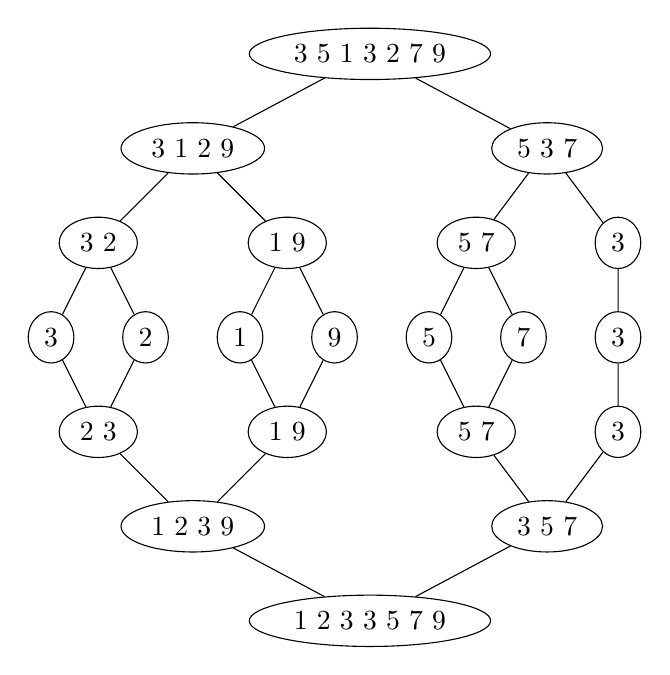
\begin{tikzpicture}[scale=1.2]
	\node [draw,ellipse] at (3.375,3) (head) {3 5 1 3 2 7 9};
	\node [draw,ellipse] at (1.5,2) (1) {3 1 2 9};
	\node [draw,ellipse] at (5.25,2) (2) {5 3 7};
	\node [draw,ellipse] at (.5,1) (3) {3 2};
	\node [draw,ellipse] at (2.5,1) (4) {1 9};
	\node [draw,ellipse] at (4.5,1) (5) {5 7};
	\node [draw,ellipse] at (6,1) (6) {3};
	\node [draw,ellipse] at (0,0) (7) {3};
	\node [draw,ellipse] at (1,0) (8) {2};
	\node [draw,ellipse] at (2,0) (9) {1};
	\node [draw,ellipse] at (3,0) (10) {9};
	\node [draw,ellipse] at (4,0) (11) {5};
	\node [draw,ellipse] at (5,0) (12) {7};
	\node [draw,ellipse] at (6,0) (13) {3};
	\node [draw,ellipse] at (.5,-1) (14) {2 3};
	\node [draw,ellipse] at (2.5,-1) (15) {1 9};
	\node [draw,ellipse] at (4.5,-1) (16) {5 7};
	\node [draw,ellipse] at (6,-1) (17) {3};
	\node [draw,ellipse] at (1.5, -2) (18) {1 2 3 9};
	\node [draw,ellipse] at (5.25, -2) (19) {3 5 7};
	\node [draw,ellipse] at (3.375,-3) (20) {1 2 3 3 5 7 9};

	\path [draw] (1) -- (head) -- (2);
	\path [draw] (3) -- (1) -- (4);
	\path [draw] (5) -- (2) -- (6);
	\path [draw] (7) -- (3) -- (8);
	\path [draw] (9) -- (4) -- (10);
	\path [draw] (11) -- (5) -- (12);
	\path [draw] (13) -- (6);
	\path [draw] (7) -- (14) -- (8);
	\path [draw] (9) -- (15) -- (10);
	\path [draw] (11) -- (16) -- (12);
	\path [draw] (13) -- (17);
	\path [draw] (14) -- (18) -- (15);
	\path [draw] (16) -- (19) -- (17);
	\path [draw] (18) -- (20) -- (19);
	\end{tikzpicture}\\*
	\newline
	Quicksort (using the first element in the list as a pivot):\\*
	\newline
	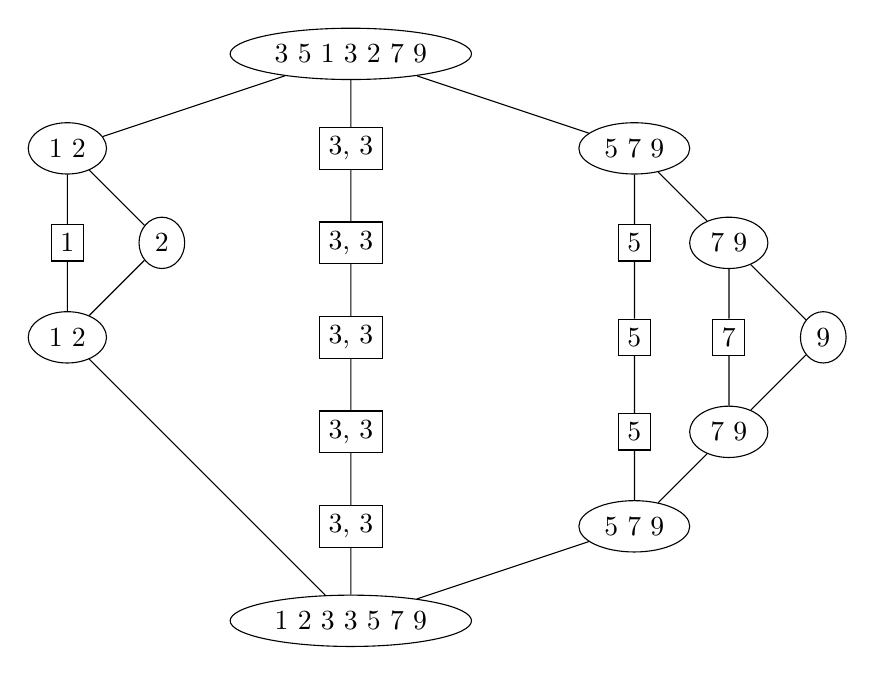
\begin{tikzpicture}[scale=1.2]
	\node [draw] at (4,0) (4) {3, 3};
	\node [draw] at (7,0) (5) {5};
	\node [draw] at (8,0) (6) {7};
	\node [draw,ellipse] at (9,0) (7) {9};
	\node [draw] at (1,1) (8) {1};
	\node [draw, ellipse] at (2,1) (9) {2};
	\node [draw] at (4,1) (10) {3, 3};
	\node [draw] at (7,1) (11) {5};
	\node [draw,ellipse] at (8,1) (12) {7 9};
	\node [draw, ellipse] at (1,2) (13) {1 2};
	\node [draw] at (4,2) (14) {3, 3};
	\node [draw,ellipse] at (7,2) (15) {5 7 9};
	\node [draw,ellipse] at (4,3) (16) {3 5 1 3 2 7 9};
	\node [draw] at (4, -1) (19) {3, 3};
	\node [draw] at (7,-1) (20) {5};
	\node [draw, ellipse] at (8,-1) (21) {7 9};
	\node [draw, ellipse] at (1,0) (22) {1 2};
	\node [draw] at (4,-2) (23) {3, 3};
	\node [draw, ellipse] at (7,-2) (24) {5 7 9};
	\node [draw, ellipse] at (4,-3) (25) {1 2 3 3 5 7 9};

	\path [draw] (8) -- (13);
	\path [draw] (8) -- (22);
	\path [draw] (9) -- (22);
	\path [draw] (9) -- (13);
	\path [draw] (4) -- (10) -- (14) -- (16);
	\path [draw] (5) -- (11) -- (15);
	\path [draw] (6) -- (12);
	\path [draw] (7) -- (12) -- (15) -- (16);
	\path [draw] (13) -- (16);

	\path [draw] (22) -- (25);
	\path [draw] (4) -- (19) -- (23) -- (25);
	\path [draw] (5) -- (20) -- (24);
	\path [draw] (6) -- (21);
	\path [draw] (7) -- (21) -- (24) -- (25);

	\end{tikzpicture}
    \end{answer}

\section*{Heaps and Heapsort}
	\item For a binary heap containing $n$ elements, what is the maximum number of
      swaps occurring after an insert operation?

    \begin{answer}
        log$_{\textrm{2}}$ (n + 1), rounded down.
    \end{answer}

	\item Given a node in an array-based binary heap at index $i$, where are the
      indices of both its children? What is the index of its parent?

    \begin{answer}
    The children are at $2i+1$ and $2i+2$. The parent is at
    $\lfloor\frac{i-1}{2}\rfloor$.

    \marginpar{\small\em Note that in a 1 indexed array system, the children
    would be at $2i$ and $2i+1$. The parent would be at
    $\lfloor\frac{i}{2}\rfloor$.}
    \end{answer}

	\item Run a heap sort in reverse order on the following list: [3,5,1,3,2,7,9], showing the heap
      at each stage. Be sure to heapify the list first.

    \begin{answer}
        Heapify:  \newline
        	[\underline{3}, 5, 1, 3, 2, 7, 9] \newline
    		[\underline{3}, \underline{5}, 1, 3, 2, 7, 9] \newline
    		[\underline{1}, \underline{5}, \underline{3}, 3, 2, 7, 9] \newline
    		[\underline{1}, \underline{3}, \underline{3}, \underline{5}, 2, 7, 9] \newline
    		[\underline{1}, \underline{2}, \underline{3}, \underline{5}, \underline{3}, 7, 9] \newline
    		[\underline{1}, \underline{2}, \underline{3}, \underline{5}, \underline{3}, \underline{7}, 9] \newline
    		[\underline{1}, \underline{2}, \underline{3}, \underline{5}, \underline{3}, \underline{7}, \underline{9}] \newline 
    	
    	Sort: \newline
    		[\underline{2}, \underline{3}, \underline{3}, \underline{5}, \underline{9}, \underline{7}, 1] \newline
    		[\underline{3}, \underline{3}, \underline{7}, \underline{5}, \underline{9}, 2, 1] \newline
    		[\underline{3}, \underline{5}, \underline{7}, \underline{9}, 3, 2, 1] \newline
    		[\underline{5}, \underline{9}, \underline{7}, 3, 3, 2, 1] \newline
    		[\underline{7}, \underline{9}, 5, 3, 3, 2, 1] \newline
    		[\underline{9}, 7, 5, 3, 3, 2, 1] \newline
    		[9, 7, 5, 3, 3, 2, 1] \newline
    \end{answer}

	
\newpage
\section*{Greedy Algorithms}
	\item Given that an algorithm is \textit{greedy}, is it guaranteed to return an \textit{optimal} solution?

\begin{answer}
NO. Greedy algorithms always choose the \textit{current} best solution,
which is not necessarily the \textit{overall} best solution!
\end{answer}

	
	\vspace{.25in}
	
	\item \textbf{Greedy algorithms.}
In the game Black and White\footnote{Special thanks to Professor Butler for unwittingly allowing us to rip off his problem.}, the player is faced with a row of identical double-sided chips.
You can probably guess what colors the two sides of each chip are.
The objective is to flip as many chips as necessary so their exposed colors match that of a target pattern. \\
The catch?
Reordering the chips is said to be Impossible by those who seem to know what they're talking about. \\
The \textit{real} catch?
Flipping a group of consecutive tiles can be accomplished in a single ``action.'' \\
If every flip takes one ``action,'' write a function \texttt{bwMoves} that, given a starting pattern and target pattern as equal-length strings, returns the minimum number of actions required to get them to match.
For instance, \texttt{bwMoves( 'BBWBBWBBBB', 'WWWWWBBWWB' )} should return 3.
\vspace{6pt} \\
\textit{Hint: Were any of the other questions labeled with the concept they were testing?}
\begin{answer}
\begin{lstlisting}
def bwMoves(start, target):
	actions=0
	first=0
	for index in range(len(start)):
		if start[index]==target[index]:
			if first!=index: # Each flip works up to (but not including)
				actions+=1	 # the index pointer. If first==index, that's
			first=index+1	 # 0 elements, so there is nothing to flip.
							 # (i.e. There were two no-flips in a row.)
	if start[-1]!=target[-1]:
		actions+=1
	return actions
\end{lstlisting}
\end{answer}

\end{enumerate}
\end{document}
